\documentclass[11pt, letterpaper]{article}
\setlength{\parindent}{0in}
\setlength{\textheight}{8.7in}
\setlength{\textwidth}{6.8in}
\setlength{\oddsidemargin}{-0.3in}
\setlength{\evensidemargin}{0.0in}
\addtolength{\topmargin}{-1in}
\setlength{\parskip}{0.1in}

\usepackage{amsmath, amsfonts, amssymb, color}
\usepackage{booktabs}
\usepackage{bm}
\usepackage{enumerate}
\usepackage{graphicx}
\newcommand*{\justifyheading}{\raggedleft}


\renewcommand{\baselinestretch}{1.0}

\newcommand{\bx}{{\bm x}}
\newcommand{\bX}{{\bm X}}
\newcommand{\by}{{\bm y}}
\newcommand{\bY}{{\bm Y}}
\newcommand{\bW}{{\bm W}}
\newcommand{\bG}{{\bm G}}
\newcommand{\bR}{{\bm R}}
\newcommand{\bZ}{{\bm Z}}
\newcommand{\bV}{{\bm V}}
\newcommand{\bL}{{\bm L}}
\newcommand{\bz}{{\bm z}}
\newcommand{\be}{{\bm e}}
\newcommand{\bgamma}{{\bm \gamma}}
\newcommand{\bbeta}{{\bm \beta}}
\newcommand{\balpha}{{\bm \alpha}}
\newcommand{\bSigma}{{\bm \Sigma}}
\newcommand{\bmu}{{\bm \mu}}
\newcommand{\btheta}{{\bm \theta}}
\newcommand{\bepsilon}{{\bm \epsilon}}
\newcommand{\bone}{{\bm 1}}
\newcommand{\bzero}{{\bm 0}}
\newcommand{\bC}{{\bm C}}
\newcommand{\bI}{{\bm I}}
\newcommand{\bA}{{\bm A}}
\newcommand{\bB}{{\bm B}}
\newcommand{\bQ}{{\bm Q}}
\newcommand{\bS}{{\bm S}}
\newcommand{\bD}{{\bm D}}
\newcommand{\cQ}{\mathcal{Q}}
\newcommand{\cU}{\mathcal{U}}
\newcommand{\cI}{\mathcal{I}}
\newcommand{\cL}{\mathcal{L}}

\newcommand{\beas}{\begin{eqnarray*}}
\newcommand{\eeas}{\end{eqnarray*}}

\newenvironment{equationarrayright}{
                          \begin{eqnarray*}
                          \begin{array}{rcll}
                         }{
                          \end{array}
                          \end{eqnarray*}
                         }
\newcommand{\bear}{\begin{equationarrayright}}
\newcommand{\eear}{\end{equationarrayright}}

\renewcommand\arraystretch{1.3}

\DeclareMathOperator*{\argmin}{arg\,min}

\title{STAT/BIOST 571: Homework 5}
\author{Philip Pham}
\date{\today}

\begin{document}

\maketitle

\section*{Problem 1: Sandwich and bootstrap standard error estimates (10 points)}
{\em As on slide 2.76, fit the model
\[
EY_{ij}=\beta_0 +\beta_1(Age_{ij}-8)+\beta_2 Gender_i + \beta_3(Age_{ij} -8)\times Gender _i
\]
to the dental data by using REML, but use a homoscedastic covariance models with no correlation.}
\begin{enumerate}[(a)]
{\em \item Calculate sandwich-based standard error estimates for $\hat{\beta_3}$ that account for clustering by subject.  Write your
  own code for this, using matrix algebra.}

\begin{table}[h]
  \centering
  \begin{tabular}{lrrr}
\toprule
{} &   Estimate &  REML Standard Error &  Sandwich Standard Error \\
\midrule
$\hat\beta_0$ &  22.615610 &             0.472075 &                 0.533556 \\
$\hat\beta_1$ &   0.784380 &             0.126167 &                 0.098347 \\
$\hat\beta_2$ &  -1.406521 &             0.739599 &                 0.773799 \\
$\hat\beta_3$ &  -0.304834 &             0.197666 &                 0.116867 \\
\bottomrule
\end{tabular}

  \caption{Parameter estimates using REML with a homoscedastic covariance models
    with no correlation.}
  \label{tab:reml_estimates}
\end{table}

\begin{description}
\item[Solution:] The REML estimates can be found in Table
  \ref{tab:reml_estimates}. Standard errors were calculated assuming that
  covariance model is specified correctly by taking the square root of the
  diagonal
  $\left(\sum_{i=1}^n X_i^\intercal \hat{\Sigma}^{-1}_{\text{REML}}
    X_i\right)^{-1}$, where $\hat{\Sigma}_{\text{REML}} = \hat{\alpha} I_m$,
  since cluster sizes are equal and there is only one covariance parameter on
  the diagonal.
  
  Sandwich covariance estimates can be obtained by
  \begin{align*}
    \hat{\Sigma}_{\text{Sandwich}}
    &=
    \left(\sum_{i=1}^n X_i^\intercal \hat{\Sigma}^{-1}_{\text{REML}} X_i\right)^{-1}
    \left(\sum_{i=1}^n X_i^\intercal\hat{\Sigma}^{-1}_{\text{REML}}
      \hat{\Sigma}_{\text{Empirical}}
      \hat{\Sigma}^{-1}_{\text{REML}}X_i\right)
    \left(\sum_{i=1}^n X_i^\intercal \hat{\Sigma}^{-1}_{\text{REML}} X_i\right)^{-1},
  \end{align*}
  where the empirical covariance estimate is
  $\hat{\Sigma}_{\text{Empirical}} = \frac{1}{n}\sum_{i=1}^n \left(Y_i -
    X_i\hat{\beta}\right)\left(Y_i - X_i\hat{\beta}\right)^\intercal$ since we
  assume each cluster has the same covariance structure.

  Using $\hat{\Sigma}_{\text{Sandwich}}$ for to get the standard error of
  $\hat{\beta}_3$, we obtain a smaller standard error $\boxed{0.11686716}$ since
  we can exploit within cluster correlation to get a better estimate.
\end{description}
{\em \item Calculate bootstrap standard error estimates 
for $\hat{\beta}_3$ by resampling clusters.  Describe the results of some basic diagnostics you can do to provide confidence that
bootstrap intervals are valid for this dataset and that you have simulated a sufficient number 
of draws to accurately approximate true bootstrap intervals?}

\begin{figure}
  \centering
  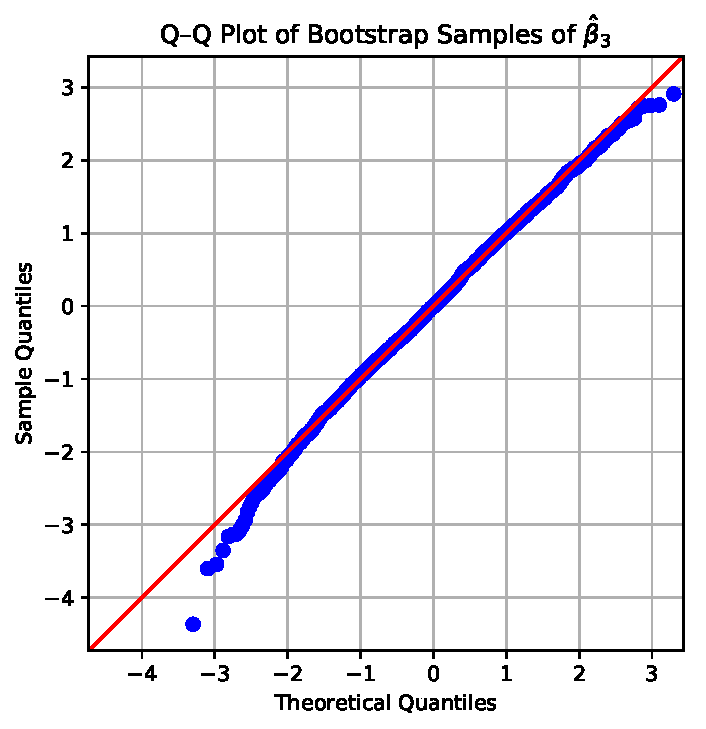
\includegraphics{qq_bootstrap_cluster.pdf}
  \caption{Bootstrap Q--Q plot for $\hat\beta_3$ when resampling clusters.}
  \label{fig:qq_bootstrap_cluster}
\end{figure}

\begin{description}
\item[Solution:] The bootstrap standard error for $\hat{\beta}_3$ when
  resampling clusters is $\boxed{0.11997406,}$ which is similar to the
  sandwich estimate.

  This was calculated by taking the square root of the sample variance of the of
  the boostrap samples for $\hat{\beta}_3$. 2,048 samples were taken. Normality
  of the samples was checked by using a Q--Q plot in Figure
  \ref{fig:qq_bootstrap_cluster} and a histogram in Figure
  \ref{fig:hist_bootstrap_cluster}. The distribution in the histrogram does look
  normal, and the fit in the Q--Q plot is quite good, so we can be confident
  that the distribution of the samples is indeed normal.

  Indeed, if $\hat{\beta}_3$ is our REML estimate, $\hat{\sigma}$ is our
  bootstrap standard error, and $\Phi$ is the CDF for the standard normal, then
  the interval
  $\left[\hat{\beta}_3 - \Phi^{-1}\left(0.975\right)\hat{\sigma}, \hat{\beta}_3
    + \Phi^{-1}\left(0.975\right)\hat{\sigma}\right]$ contains 94.97\% of the
  bootstrap samples, so the interval is quite accurate.
\end{description}

\begin{figure}
  \centering
  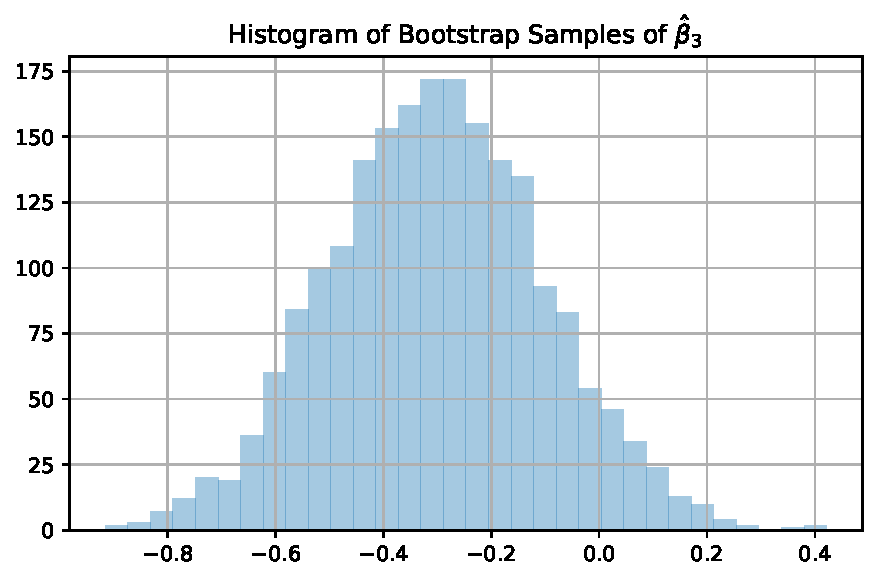
\includegraphics{hist_bootstrap_cluster.pdf}
  \caption{Bootstrap histogram for $\hat\beta_3$ when resampling clusters.}
  \label{fig:hist_bootstrap_cluster}
\end{figure}

{ \em \item Calculate bootstrap standard error estimates for $\hat{\beta}_3$ based on resampling observations
without regard to cluster and resampling both clusters and observations within clusters. }
{\em \item Discuss any differences between your sandwich standard error estimates and the three versions of bootstrap standard errors.}
\end{enumerate} 



\end{document}